\documentclass[10pt, letterpaper]{memoir}
\usepackage{HWStyle}
\usepackage{mdframed}

\begin{document}
	\begin{center}
		{\Huge CHEM 3610}
		{\LARGE-- Fall 2016
		
		Homework 5 Supplemental Problem
		
		Due: September 26, 2016}
	\end{center}
	
	\begin{minipage}[c]{0.55\textwidth}
		\section*{Tunneling and STM}
		A scanning tunneling microscope relies on the phenomenon of quantum tunneling to generate micrographs of a sample's electron density at atomic resolutions. Tunneling is represented schematically at right.
		
	
		Remember that the form of $\Psi$ within the potential energy barrier is an exponential decay function:
		\begin{equation}
			\Psi(x) = Ce^{-kx}
		\end{equation}
		Where the decay length $k^{-1}$ is given by:
		\begin{equation}
			\hspace{1em}k^{-1}=\sqrt{\frac{\hbar^2}{2m\left(V_0-E\right)}}
		\end{equation}
		If the barrier width is n times the decay length, then the other side of the barrier will have amplitude $\dfrac{1}{e^n}$, which is simply a restatement of equation 1 above.
		
		For a typical STM the height of the potential energy barrier $V_0$ is closely approximated by the average of $\phi_{tip}$ and $\phi_{sample}$, the work functions of the tip and sample. The energy is usually negligibly small.
		
		STMs sometimes use a gold tip ($\phi_{Au}\approx 5.25 eV$), and in our case we will be imaging a flat surface of copper atoms ($\phi_{Cu} \approx 4.80 eV$) with a step edge like that shown at right. 
		
		\begin{enumerate}
			\item What is the decay length in this case? You may need to use the conversion $1eV = 1.6\times 10^{-19} J$.
			\vspace{3em}
			\item If copper has a lattice constant of $3.597$ \r{A} and a face-centered cubic (FCC) crystal structure, what is the height of a single layer of copper atoms?
			\vspace{3em}
			\item What change in the current would be observed as the STM tip moves over the step edge?
		\end{enumerate}		
	\end{minipage}	
	\hspace{1.5em}
	\begin{minipage}[c]{0.4\textwidth}
		\begin{mdframed}
		\centering\includegraphics[width=\textwidth]{../../Quantum_Resources/Ch05/05_10_Figure}
		
		Quantum Tunneling
		\end{mdframed}
				
		\begin{mdframed}
		\centering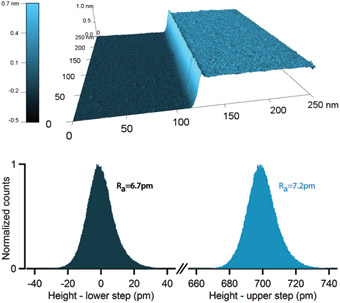
\includegraphics[width=\textwidth]{Step}
		
		A Step Edge
		\end{mdframed}
				
		\begin{mdframed}
		\centering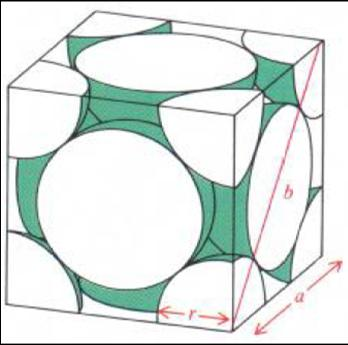
\includegraphics[width=\textwidth, trim={.1cm 0.1cm 0.1cm 0.1cm},clip]{FCC}
		
		FCC Unit Cell
		\end{mdframed}
	\end{minipage}
\end{document}
	